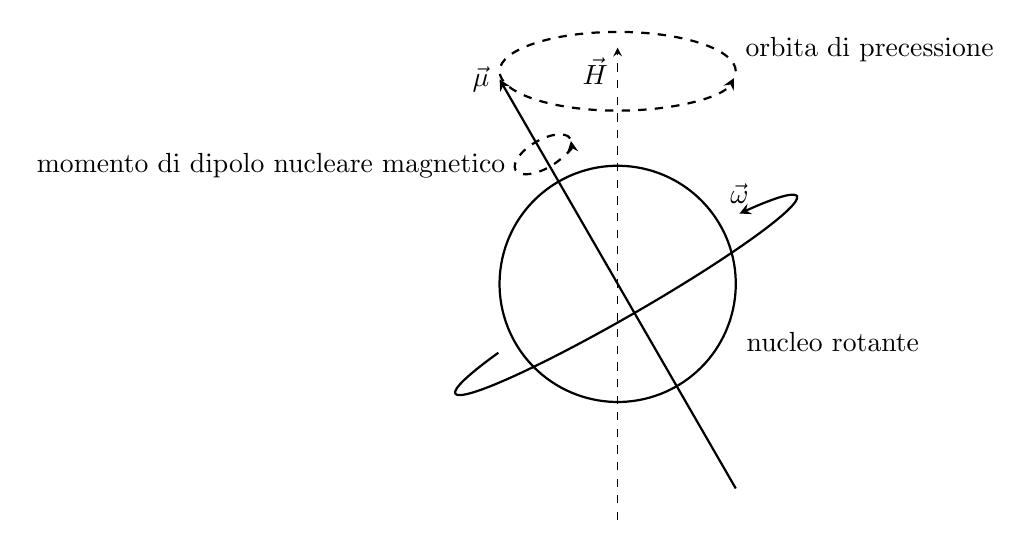
\begin{tikzpicture}[>=stealth]
% Linea tratteggiata NON ruotata
\draw[->, dashed] (0,-3)--(0,3) node[below left] {$\vec{H}$};; % al centro del cerchio
% Ellisse orientata in alto con centro sull'asse tratteggiato
\draw[dashed, thick, ->] (1.5,2.7) arc[start angle=0, end angle=350, x radius=1.5cm, y radius=0.5cm];
\node[above right] at (1.5,2.7) {orbita di precessione};

\node[right] at (-7.5,1.5) {momento di dipolo nucleare magnetico};

% Tutto il resto ruotato di 30°
\begin{scope}[rotate=30]
\shade[opacity=0] (0,0) circle(1.5); 
\draw[thick] (0,0) circle(1.5); 
\node at (2,-2) {nucleo rotante};

\draw[thick, ->] (0,-3)--(0,3) node[left] {$\vec{\mu}$};
\draw[->, dashed, thick] (0.4,1.9) arc[start angle=0, end angle=350, x radius=0.4cm, y radius=0.18cm];


\draw[thick, ->] (180:1.75) arc[start angle=135, end angle=405, x radius=2.5cm, y radius=0.25cm] node[above] {$\vec{\omega}$};
\end{scope}
\end{tikzpicture}